\documentclass[mathserif]{beamer}
\usepackage{mathtools}
\usepackage{amssymb}
\usepackage{bm}
\usepackage{graphicx}
\usetheme{Copenhagen}

\begin{document}
    \title[Analyzing Stochastic Time-Series Data]{Techniques for Analyzing Stochastic Time-Series Data}
    \author[Castleberry \and Oubre \and Yu]{Dennis Castleberry \and Brandon Oubre \and Haikou Yu}
    \date{\today}
    \frame{\titlepage}


    \section{Project Overview}
    \frame{ \frametitle{Project Overview}
        \begin{itemize}
            \item Time series data is time-ordered, with each data entry at a later time step or stamp.
            \item Given a prediction task, unlike with regular data sets, the order of the data matters; e.g. using previous time-ordered values to predict the next value in a series.
            \item Given all time-dependent data up to a certain point, our task is to predict the class value for the next time step.
            \item Our project examines feature extraction on multivariate stochastic time series data  to maximize classification accuracy for various classifiers (Naive Bayes, neural network, SVM, KNN, and CART).
            \item How can we do feature extraction on attribute values for previous time steps to achieve accurate predictions?
        \end{itemize}
    }


    \frame{ \frametitle{Project Overview}
        \begin{itemize}
            \item For our base model, we use the raw attribute set. We use this
	      model as a comparison for our other models.
            \item To generate other models, we improve add attributes to current data 
	      from previous data.
            \item For example, we hypothesize: does informing a classifier of the class of the
	      previous \(n\) entries improve prediction accuracy for the
	      current observation? We create a model wherein our derived attributes consist
	      of the class values for the previous $n$ entries.
            \item Our overarching goal is to find the relationship between classifier
	      accuracy and how much previous data to include; what are the trade-offs 
	      of deriving large amounts of data; how should the data be incorporated.
        \end{itemize}
    }


    \section{Background}
    \subsection{Naive Bayes}
    \subsubsection{Overview}
    \frame{ \frametitle{The Naive Bayes Classifier}
        \begin{itemize}
            \item Reduce classification to a computation of probabilities. What is \(P(class | attribute1, attribute2, ..., attributeN)\).
            \item Assumes that each attribute is independent of the others. (Hence the ``Naive'' nickname.)
            \item For example, let's consider if a car is stolen using \(P(stolen |
	      Color, Type)\). Naive Bayes will assume \(color=red\) and
	      \(type=sportscar\) to be independent.
        \end{itemize}
    }


    \subsubsection{Example}
    \frame{ \frametitle{Naive Bayes in Action}
        \begin{center} 
            \textbf{Training Data} \\
            \begin{tabular}{c | c | c || c}
                \textbf{Over 170cm} & \textbf{Eye Color} & \textbf{Hair Length} & \(\boxed{\textbf{Sex}}\) \\ \hline \hline
                No & Blue & Short & Male \\ \hline
                Yes & Brown & Long & Female \\ \hline
                No & Blue & Long & Female \\ \hline
                Yes & Brown & Short & Male \\ \hline
                Yes & Brown & Short & Female \\
            \end{tabular}  \\
            \small{Only discrete values shown, but we can still apply numeric data using standard deviations if the data is normally distributed.}
        \end{center}
            Suppose we are given an unseen data point \(\langle No, Blue, Short \rangle\). What should we classify it as?
    }


    \frame{ \frametitle{Naive Bayes in Action}
        \begin{tabular}{l}
        \(P(Male|No,Blue,Short)\) \\
        \(=\dfrac{P(No,Blue,Short|Male) P(Male)}{P(No,Blue,Short)}\) \\
        \(= \alpha P(Male)\bm{P(No|Male)P(Blue|Male)P(Short|Male)}\) \\
        \(=\alpha \times \frac{2}{5} \times \frac{1}{2} \times \frac{1}{2} \times \frac{2}{2} = \boxed{0.1\alpha}\) \\ \\
        \hline \\
        \(P(Female|No,Blue,Short)\) \\
        \(=\alpha P(Female)P(No|Female)P(Blue|Female)P(Short|Female)\) \\
        \(= \alpha \times \frac{3}{5} \times \frac{1}{3} \times \frac{1}{3} \times \frac{1}{3} = \boxed{0.0\overline{2}\alpha}\) \\
        \end{tabular} \\
        \vspace{10px}
        Since \(P(Male|Data) > P(Female|Data)\), we classify the unseen point as Male. For multiple classes, just select the class with the greatest probability!
    } 


    \subsection{Support Vector Machine}
    \subsubsection{Overview}
    \frame{ \frametitle{Support Vector Machines (SVM)}
        \begin{itemize}
            \item Idea is to draw a line (or hyperplane) between the data points of
	      different classes. Classify unseen data by testing which side of
	      the line it is on.
            \item Focus on support vectors, or the points that would change the
	      line if removed from the training data.
            \item Find an optimal line to separate the data. Such a line will have
	      the larger margin for data points and should mis-classify the
	      least number of new points.
            \item If data is not linearly separable, then a transformation of the
	      data to a new basis can be performed. The data may be linearly
	      separable in the new basis.
        \end{itemize}
    }


    \subsubsection{Example}
    \frame{ \frametitle{SVM Example}
        \begin{columns}[t]
            \column{.5\textwidth}
            \begin{figure}
                \centering
                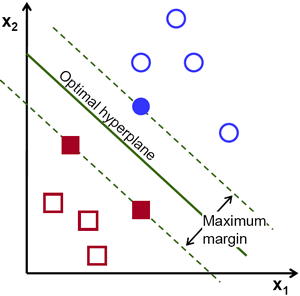
\includegraphics[keepaspectratio,scale=2]{SVM.png} \\ \vspace{5px}
                \Tiny{Image from \url{http://docs.opencv.org/doc/tutorials/ml/introduction_to_svm/introduction_to_svm.html}}
            \end{figure}
            
            \column{.5\textwidth}
            \begin{itemize}
                \item Solid points are support vectors.
                \item With a maximized margin, unseen figures closer to
		  the line than the support vectors are still correctly
		  classified.
                \item It is easy to see how new points are classified.
            \end{itemize}
        \end{columns}
    }


    \subsection{Neural Network}
    \subsubsection{Overview}
    \frame{ \frametitle{Neural Networks}
        \begin{itemize}
            \item Inspired by biological neurons.
            \item Neurons maintain a weighted sum of their inputs. The result of
	      this sum is passed into a function and output. (A step function
	      produces on/off signals while a Sigmoid will produce continues
	      levels of activation.)
            \item The network can be trained by adjusting the weights of the inputs to each neuron.
            \item In a feed-forward network, the backwards propagation algorithm accomplishes this.
            \item Networks with multiple layers can classify various types of non-linearly separable data.
        \end{itemize}
    }


    \subsubsection{Structure and Classification}
    \frame{ \frametitle{An Artificial Neuron}
        \begin{figure}
            \centering
            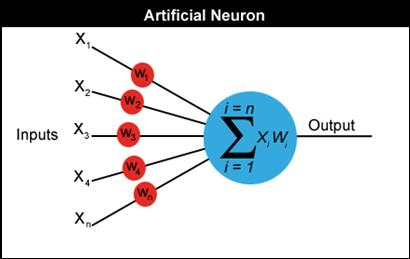
\includegraphics[keepaspectratio,scale=.9]{NN_1.jpg} \\
            \Tiny{Image from \url{http://www.ai-junkie.com/ann/evolved/nnt1.html}}
        \end{figure}
    }


    \frame{ \frametitle{Neural Network Classification}
        \begin{columns}[t]
            \column{.5\textwidth}
            \begin{figure}
                \centering
                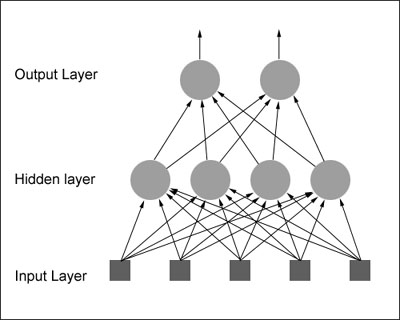
\includegraphics[keepaspectratio,scale=0.4]{NN_2.jpg} \\ \vspace{5px}
                \Tiny{Image from \url{http://www.ai-junkie.com/ann/evolved/nnt1.html}}
            \end{figure}
            
            \column{.5\textwidth}
            \begin{itemize}
                \item Information is fed into the input layer.
                \item The outputs of the neurons in the output layer represent predicted class values.
            \end{itemize}
        \end{columns}
    }


    \subsection{K-Nearest Neighbor (KNN)}
    \subsubsection{Overview}
    \frame{ \frametitle{K-Nearest Neighbor}
        \begin{itemize}
            \item Assumes that data vectors lie in a metric space (a distance measure can
	      be computed).
            \item Classification is simple. To classify point \(x\), find the
	      k points in the training data closest to \(x\). Classify \(x\) as
	      the majority vote of its k-nearest neighbors' class.
            \item Can also weight votes based on the distance of the neighbors.
        \end{itemize}
    }


    \subsubsection{Example}
    \frame{ \frametitle{KNN Example}
        \begin{columns}[t]
            \column{.5\textwidth}
            \begin{figure}
                \centering
                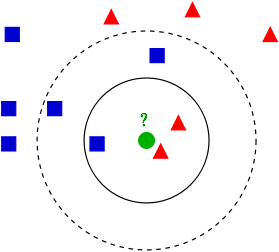
\includegraphics[keepaspectratio,scale=0.5]{KNN.png} \\ \vspace{5px}
                \Tiny{Image from \url{http://en.wikipedia.org/wiki/File:KnnClassification.svg}}
            \end{figure}
            
            \column{.5\textwidth}
            \begin{itemize}
                \item Red and blue points represent training data.
                \item The green point is being classified.
                \item For \(k=3\) the point is classified as red.
                \item For \(k=5\) the point is classified as blue.
                \item Weighting votes by distance may shift favor back to red.
            \end{itemize}
        \end{columns}
    }


    \subsection{CART}
    \subsubsection{Overview}
    \frame{ \frametitle{Classification and Regression Tree (CART)}
        \begin{itemize}
            \item Create binary decision trees. Minimize the error in each leaf.
            \item Produces a classification tree for categorical data and a regression tree for numerical data.
            \item Data is recursively split according to rules until a set of stopping rules are met or when no further gain can be made.
            \item Can also split data as much as possible and the prune.
            \item Each internal node is a decision.
            \item Each leaf is a classification, which classifies according to majority vote of training data that follows that tree path.
        \end{itemize}
    }

    \subsubsection{Example}
    \frame{ \frametitle{CART Example}
        \begin{columns}[t]
            \column{.5\textwidth}
            \begin{figure}
                \centering
                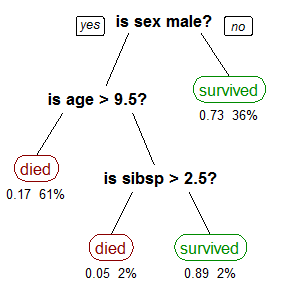
\includegraphics[keepaspectratio,scale=0.5]{CART.png} \\ \vspace{5px}
                \Tiny{Image from \url{http://en.wikipedia.org/wiki/File:CART_tree_titanic_survivors.png}}
            \end{figure}
            
            \column{.5\textwidth}
            \begin{itemize}
                \item CART tree for classifying survival of passengers on the Titanic.
                \item Sibsp is number of spouses and siblings aboard the ship.
                \item Tree also shows probability of survival and percentage of observations.
                \item To classify unseen data point simply follow the tree until a leaf node is met.
            \end{itemize}
        \end{columns}
    }


    \section{Experimental Design}
    \subsection{Setup}
    \frame{ \frametitle{Experiment Setup}
        \begin{itemize}
            \item We are given a time series \(T\) where each entry has attributes \(A_1, A_2, ..., A_N\) and classes value \(C\).
            \item Cannot use k-fold cross-validation. \\
                \begin{itemize}
                    \item Data order not interchangeable.
                    \item Must predict future entry given past entries.
                    \item The more unseen data we use to make predictions, the less accurate future predictions become. (Think of weather predictions.)
                \end{itemize}
            \item Solution: Split series up into partitions of size \(M\). Train
	      model on data entries \(1, 2, ..., (M-1)\) and predict unseen
	      entry \(M\). Tally up number of correct predictions from all
	      partitions in the data set to determine accuracy.
        \end{itemize}
    }


    \frame{ \frametitle{Experimental Conjecture}
        \begin{itemize}
            \item Since the time series is stochastic, the attributes and class
	      values of \(T[1:i-1]\) may influence the attribute and class
	      values of \(T[i]\).
            \item Our conjecture is that adding derived attributes to each
	      element's native attributes can improve classification accuracy.
	      These derived attributes contain information about previous
	      elements in the time series, which gives them predictive power.
            \item For example, the average weather conditions over the past 10
	      minutes could help predict the weather condition one minute from
	      now.
        \end{itemize}
    }


    \subsection{Design}
    \frame{ \frametitle{Experiment Design}
        \begin{itemize}
            \item Establish hypothesis \(H_0\), which is a classification task done on the raw data set (No derived attributes).
            \item Create hypotheses \(H_1, H_2, ..., H_N\), which each add different sets of derived attributes to the raw data.
            \item Run each \(H_i\) through the same classifier and observe the difference in classifier accuracy.
            \item Repeat this process for new hypotheses and different classifiers.
            \item Analyze results to determine which Hypotheses perform better with which classifiers, if any.
        \end{itemize}
    }

    \subsection{Hypotheses}
    \frame{ \frametitle{Hypotheses}
        \begin{itemize}
            \item In \(H_1\) we use as a derived attribute the class value from the previous iteration.  We simply copy the
	      class as an attribute of the data set and shift the column up by one.
            \item In \(H_2\) we use as derived attributes the previous values for the native attributes. To do so, we simply
	      copy the attribute data set and shift the column up by one.
            \item \(H_3\) is similar to \(H_2\) but uses $m$ previous rows of the data.
            \item In \(H_4\) we use as derived attributes simple moving averages (MAs) of the previous $m$ values.  If $i$ is the
	      index of the current datum for a given attribute, we define the MA as $\sum_{j=1}^m \alpha_j x_{i-j}$. For a simple
	      moving average, all $\alpha$'s have equal weights.
            \item In \(H_5\) we use as derived attributes exponential moving averages (MAs) of the previous $m$ values.   For an 
	      exponential moving average, all $\alpha$'s have weights which are proportional to $i$. 
        \end{itemize}
    }


    \subsection{Data}
    \frame{ \frametitle{Data}
        \begin{itemize}
            \item ISTANBUL STOCK EXCHANGE Data Set 
	    \item Attributes: day, month, year, ISE, SP, DAX, FTSE, NIKKEI, BOVESPA, EU
	    \item Class: EMI up/down.
	    %\item C Paper: Akbilgic, O., Bozdogan, H., Balaban, M.E., (2013) A novel Hybrid RBF Neural Networks model as a forecaster, Statistics and Computing. DOI 10.1007/s11222-013-9375-7 
            %PhD Thesis: Oguz Akbilgic, (2011) Hibrit Radyal Tabanlı Fonksiyon Ağları ile Değişken Seçimi ve Tahminleme: Menkul Kıymet Yatırım Kararlarına İlişkin Bir Uygulama, Istanbul University
        \end{itemize}
    }
    \frame{ \frametitle{Data}
        \begin{itemize}
            \item  EEG Eye State Data Set 
            \item  All data is from one continuous EEG measurement with the Emotiv EEG Neuroheadset. The eye state was detected via a camera during the EEG measurement and added later manually to the file after analysing the video frames. 
	    \item  Attributes: EEG electrode potentials.
	    \item  Class: Eyes open/closed.
	 \end{itemize}
    }

    \subsection{Data}
    \frame{ \frametitle{Data}
        \begin{itemize}
            \item Diabetes Data Set 
            \item Attributes: month, day, hour, minute.
            \item Class: normal/abnormal.
        \end{itemize}
        \begin{itemize}
            \item Power Consumption Data
            \item Attributes: day, month, year, hour, minute, second, reactive, voltage
            \item Class: normal/abnormal.
        \end{itemize}
    }

    \section{Implementation}


    \section{Experimental Results}
    \frame{ \frametitle{\(H_1\) Results}
        \begin{center}
            \begin{tabular}{l | l | c | c}
                \textbf{Data Set} & \textbf{Classifier} & \textbf{\(H_1\) Acc} & \textbf{\(H_0\) Acc} \\ \hline
                Sample & Naive Bayes & x\% & y\% \\
                Sample & SVM & x\% & y\% \\
                Sample & Neural Net & x\% & y\% \\
                Sample & KNN & x\% & y\% \\
                Sample & CART& x\% & y\% \\
            \end{tabular}
        \end{center}
    }


\end{document}
